% ======================================================================
% Euclid Strong Lensing Science Working Group White Paper
% ======================================================================

\documentclass[twocolumn]{svjour3}

\usepackage[utf8]{inputenc}
\usepackage{natbib}
\usepackage{graphicx}
\usepackage{layout}
\usepackage{amsmath}
\usepackage{amssymb}

\def\apj{ApJ}

% ======================================================================

\begin{document}

\title{Euclid Science with Strong Gravitational Lenses}
\titlerunning{Euclid Science with Strong Gravitational Lenses}

\author{The Euclid Consortium Strong Lensing Science Working Group:\\
Tom Collett$^1$ \and
Remi Cabanac \and
Frederic Courbin \and
Giovanni Covone \and
Pierre Dubath \and
Alexander Fritz \and
Raphael Gavazzi \and
Carlo Giocoli \and
Philippa Hartley \and
Neal Jackson \and
Eric Jullo \and
Steve Kahn \and
Gijs Verdoes Kleijn \and
Jean-Paul Kneib \and
Leon Koopmans \and
Eric Linder \and
Phil Marshall$^4$ \and
Massimo Meneghetti \and
R. Benton Metcalf \and
Leonidas Moustakas \and
Enrico Petrillo \and
Stephen Serjeant \and
Dominique Sluse \and
Amitpal Tagore \and
Andrea Tramacere \and
Giorgos Vernardos
}
\authorrunning{Euclid Strong Lensing Science Working Group}

\institute{%
$^1$ ICG, Portsmouth, UK. \\
$^4$ KIPAC, Stanford, CA, USA. \\
\email{ecsls@groups.google.com}
}


\maketitle

% ----------------------------------------------------------------------

\begin{abstract}
\noindent Euclid will image \emph{a lot of sky} at \emph{high
resolution}. This dataset will contain {\it a large number} of lenses of
various types, enabling a variety  of different  science investigations.
In this white paper we describe a set of key projects, that exercise the
unique capability of Euclid coupled to a large array of gravitational
lenses, that we plan to carry out using the Euclid dataset, outlining
the motivation, expectations and technical challenges associated with
each one.
\keywords{surveys -- techniques \and high angular resolution -- optical}
\end{abstract}


\subsection*{Paper Production Timeline}
\begin{itemize}
    \item {\bf Skeleton: October 5} (Bulleted lists of subsection contents.)
    \item {\bf First Draft: December 19} (So we can read it over the holiday.)
    \item {\bf One Month Warning: January 16} (What still needs to be done?)
    \item {\bf Complete Draft: EC Meeting, February 15} (For finalization in Bern.)
    \item {\bf Submission to arxiv: March 1} (In time for funding deadline.)
\end{itemize}


% ----------------------------------------------------------------------

\section{Introduction}

{\it Responsible: Fred}

Strong lensing as a tool for studying the universe and its contents.
Unique capabilities of Euclid coupled to strong lenses. How our  work
fits with other working groups.

Why are we writing this paper? And why are we writing it now?

Technical challenges. History of finding, challenge of Euclid. History
of  measurement/modeling, challenge of Euclid.

Goals of this paper.

This paper is organized as follows. In Section~\ref{sec:yield} we assess
the  potential of the Euclid dataset, calculating the expected abundance
of a  number of different strong gravitational lenses detectable with
Euclid. With  this in hand, we then  describe, in
Sections~\ref{sec:astrophysics} and~\ref{sec:cosmology}, a set  of
strong lensing science projects that we plan to do using the Euclid
data.

% ----------------------------------------------------------------------

\section{Survey Yield}

\subsection{Galaxies}
\noindent{\it Contributors: Leon Koopmans, Massimo Meneghetti, Tom Collett, Enrico Petrillo}

\begin{figure*}[t]
\centering
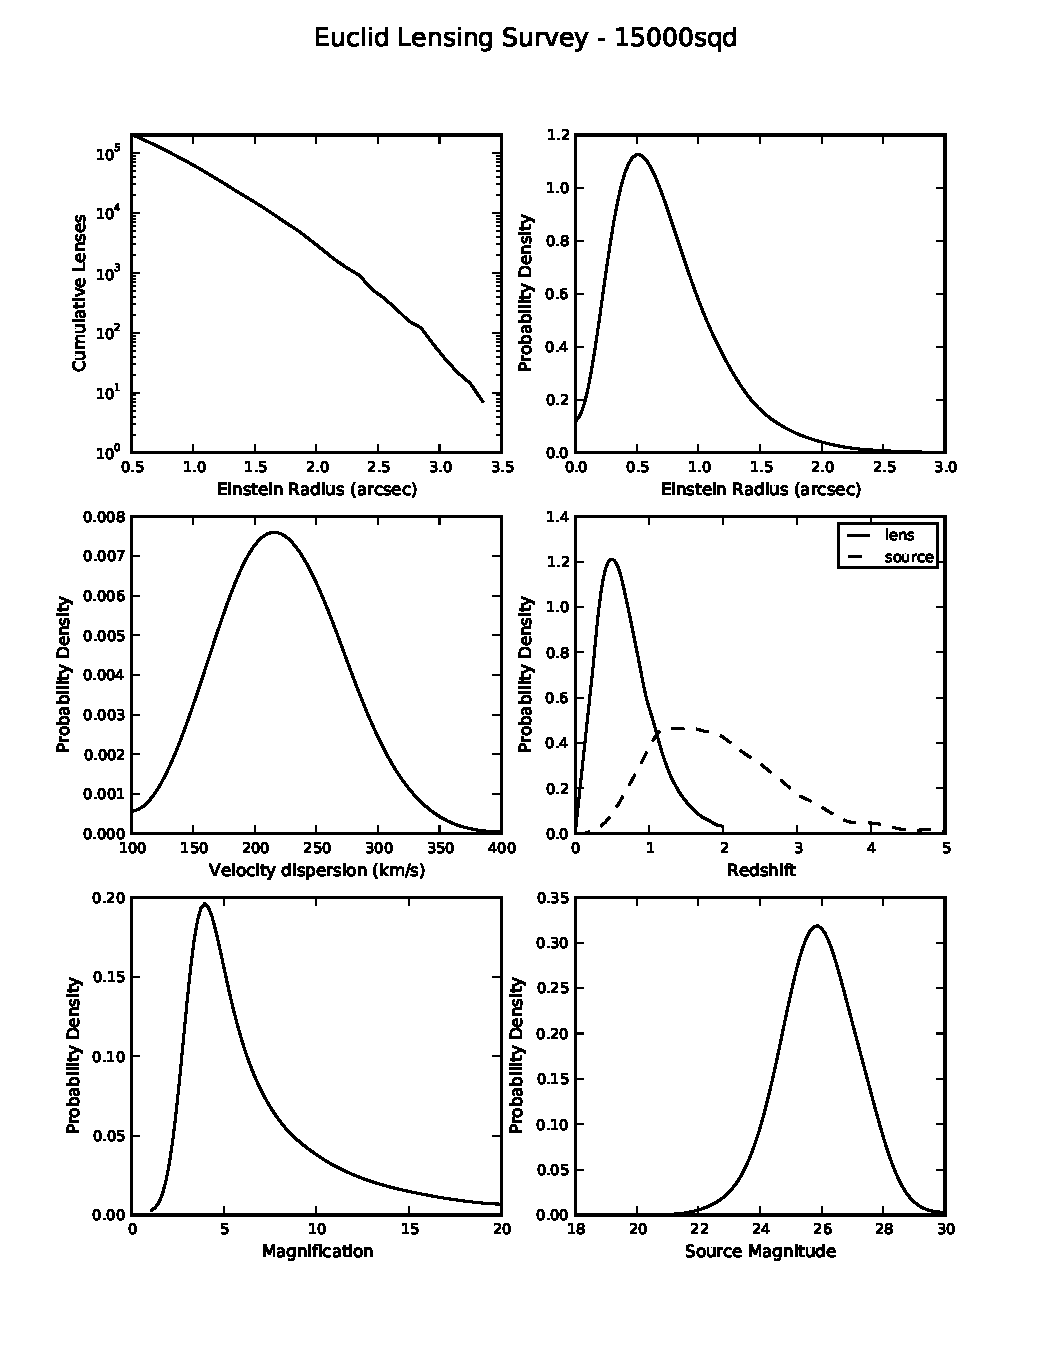
\includegraphics[width=0.7\hsize]{allplots_Euclid-3.pdf}
\caption{Expected number of lenses and their properties in the Euclid shallow survey.}
\end{figure*}

\noindent{\it Responsible: Leon}

Galaxy-scale = anything with $ M_{\odot} < 10^{12}$

\subsection{Groups and cluster}

\noindent{\it Responsible: Max}

Groups, clusters $ 10^{13}< M_{\odot} < 10^{15}$

Forecasts for lens numbers, of various kinds, to various signal-to-noise ratios.

Subsamples that science will depend on.

For deep fields, wide fields.

We use the {\sc LensPop} package by \citet{Collett2015} to make
forecasts.

\subsection{Miscellaneous}

\noindent{\it Responsible: Stephen}

% ----------------------------------------------------------------------

\section{Astrophysics}



Preamble.


% - - - - - - - - - - - - - - - - - - - - - - - - - - - - - - - - - - -

\subsection{Structure and Evolution of Galaxies}
\label{sec:lensgalaxies}

\noindent{\it Contributors: Amit Tagore, Neal Jackson, Leon Koopmans,
Dominique Sluse, Giorgos Vernardos, Raphael Gavazzi, Frederic Courbin,
Philippa Hartley, Ben Metcalf}

\noindent{\it Responsible: Leon}

Preamble.\footnote{Subsection~\ref{sec:lensgalaxies} could potentially
get very large. We may need to split it up into several different
science cases, led by different people.}

\subsubsection{Motivation}
Current state of the art. Science questions.\\

\subsubsection{Expectations}
Improvements with Euclid.\\

\subsubsection{Technical Challenges}
What do we need to do between now and first light?\\
Notes on lens finding for this science case.\\
Notes on lens measurement.\\
Notes on follow-up observations and synergies with other surveys: radio
(Philippa) \\
Notes on inference.\\

% - - - - - - - - - - - - - - - - - - - - - - - - - - - - - - - - - - -

\subsection{Structure and evolution of galaxy clusters and groups}

\noindent{\it Contributors: Raphael Gavazzi, Massimo Meneghetti, Jean-Paul Kneib, R Cabanac, Alexander Fritz}\\
\noindent{\it Responsible: Massimo}

Preamble.

\subsubsection{Motivation}
Current state of the art. Science questions.\\

\subsubsection{Expectations}
Improvements with Euclid.\\

\subsubsection{Technical Challenges}

What do we need to do between now and first light?\\

Notes on lens finding for this science case.\\

Notes on lens measurement.\\

Notes on follow-up observations and synergies with other surveys.\\

Notes on inference.\\


% - - - - - - - - - - - - - - - - - - - - - - - - - - - - - - - - - - -

\subsection{Ultra High Redshift sources}

\noindent{\it Contributors: Stephen Serjeant, Giovanni Covone, Phil
Marshall}

\noindent{\it Responsible: Stephen}

Preamble.

\subsubsection{Motivation}
Current state of the art. Science questions.\\

\subsubsection{Expectations}

Improvements with Euclid.\\

On top of the general increase in sample size of magnified high redshift
galaxies, we expect to find a number of very highly magnification
systems where the source happens to lie on or close to a caustic
catastrophe (eg Orban de Xivry \& Marshall). Such exotic lensing events
might be expected to occur most frequently in complex group and cluster
lens systems, and lead to image distortions not commonly seen.

\subsubsection{Technical Challenges}

What do we need to do between now and first light?\\

Notes on lens finding for this science case.

Finding exotic lenses presents a different challenge. The arcs and
counter-images in higher-order catastrophes may not look appear
tangentially elongated to the visible lens; instead inner rings are
possible deltoid patterns. One strategy could be to first identify all
groups and clusters through their members' optical colors and
brightnesses alone, and then search the cutout catalogs and images of
them for lensed features. Visual inspection may well prove important
here, although re-training our machines to focus on exotica may also
prove workable.


Notes on lens measurement: modeling groups and clusters for use as
cosmic telescopes.

Notes on follow-up observations and synergies with other surveys.\\

Notes on inference.\\


% - - - - - - - - - - - - - - - - - - - - - - - - - - - - - - - - - - -

\subsection{AGN and Their Hosts}

\noindent{\it Contributors: Giorgos Vernardos, Dominique Sluse, Phil
Marshall, Leonidas Moustakas, Frederic Courbin, Ben Metcalf}

\noindent{\it Responsible: Giorgos}

Currently there are $\sim$100 known lensed quasars.
Euclid is expected to bring this number up to ??? (see section 2.1 by Leon).
Lensed quasars can be used to measure time delays (see section 4).
LSST will provide sufficient monitoring for doing this, but not sufficient resolution for accurate lens models, which Euclid can do.
Euclid will not provide light curves of quasars, but could provide multi-wavelength snapshots which could be used together with microlensing techniques to constrain AGN structure like the Broad Line Emission and even the accretion disc (e.g. see Bate 2008, O'Dowd 2015, Jimenez-Vicente 2015).
Euclid can find more lenses than LSST because of the higher resolution, despite the deeper and longer in time coverage of LSST.

\subsubsection{Motivation}
Current state of the art. Science questions.\\


\subsubsection{Expectations}
Improvements with Euclid.\\

\subsubsection{Technical Challenges}

What do we need to do between now and first light?\\

Notes on lens finding for this science case. Tuning finders for
quasars\\

Notes on lens measurement.\\

Notes on follow-up observations and synergies with other surveys.
Overlap with LSST.\\

Notes on inference.\\



% ----------------------------------------------------------------------
% The section Cosmology should be structured the same way the
% astrophysics section is, instead of being structure by techniques
% ----------------------------------------------------------------------
%
%\section{Alternative section for Cosmology}
%
%\subsection{The dynamics of the universe}
%
%\subsection{}
%

\section{Cosmology}
\label{sec:cosmology}

\noindent{\it Contributors: Ben Metcalf, Eric Linder, Tom Collett}

\noindent{\it Responsible: Phil}

While strong lensing is not a primary Euclid cosmological probe, in the
era of systematics-limited cosmology it is interesting to explore
possibilities that lead to competitive, complementary and independent
constraints. Below, we discuss the potential of Euclid cluster arc
statistics as an alternate route to the evolving cluster mass function,
and also the use of large numbers of multiple source-plane ``compound
lenses'' as cosmic rulers.\footnote{Section~\ref{sec:cosmology} may need
more subsections, let's see.}

% - - - - - - - - - - - - - - - - - - - - - - - - - - - - - - - - - - -

\subsection{Cluster Abundance}

\noindent{\it Contributors: Carlo Giocoli, Massimo Meneghetti}

\noindent{\it Responsible: Carlo}

Arc statistics, mass function.

Preamble.

\subsubsection{Motivation}
Current state of the art. Science questions.\\

\subsubsection{Expectations}
Improvements with Euclid.\\

\subsubsection{Technical Challenges}

What do we need to do between now and first light?\\

Notes on lens finding for this science case.\\

Notes on lens measurement.\\

Notes on follow-up observations and synergies with other surveys.\\

Notes on inference.\\


% - - - - - - - - - - - - - - - - - - - - - - - - - - - - - - - - - - -

\subsection{Compound Lens Cosmography}

\noindent{\it Contributors: Phil Marshall, Tom Collett, Eric Jullo, Ben Metcalf}

\noindent{\it Responsible: Tom}\\

Gravitational lens systems with multiple sources at different redshifts can, in principle, be used as cosmographic probes. Since it is (nearly) the same mass distribution that is causing the multiple imaging of all the background sources, the distance ratios associated with all the sources must be consistent. In practice there are complications, but one might hope that joint analysis of a sample of systems would ameliorate them. In this section we consider both galaxy-scale and cluster-scale compound lenses as seen by Euclid, and explore the possibility of constraining cosmological parameters with them.

\subsubsection{Motivation}

\begin{itemize}
\item The current state of the art: individual systems, gilded with a lot of high quality follow-up data. The Jackpot (Gavazzi et al, Collett+Auger) at galaxy scale. The Frontier Fields clusters (Jullo et al, Natarajan et al).
\item Science questions: 1) How is the expansion of the Universe accelerating? Compound lenses are a geometric/kinematic probe of cosmology, to first order independent of the growth of structure. 2) What are the primary residual systematic errors associated with this probe, and how are they correlated with residual systematics in other probes?
\end{itemize}

\subsubsection{Expectations}

Improvements with Euclid: Euclid should enable the construction of a
sample of $\sim100$ galaxy-scale systems, when combined with deep
ground-based imaging from LSST to obtain optical colors of the faint
imaged features. Still greater numbers of clusters and groups should be
detectable. Combined, this sample could provide competitive and
complementary constraints on the parameters of the accelerating
expansion.

Figure: distribution of Euclid compound lens $z_d - z_s$ pairs, showing
both ``galaxy-scale'' and ``cluster-scale'' systems. The clusters will
appear as ``fingers,'' with many source redshifts at each constant
cluster $z_d$. The point of this plot is to show the redshift coverage,
and also the relative contribution of the Jackpots and clusters.

Figure: some estimate of the potential constraints on cosmological
parameters from galaxy-scale and cluster-scale lenses, presumably given
optimistic predictions of the impact of line of sight structure....


\subsubsection{Technical Challenges}

What do we need to do between now and first light?\\

Finding compound lenses will depend on our being able to detect the
fainter secondary arcs, potentially in the presence of confusing
foreground lens light. Color separation will be important: we must be
able to detect lensed features at low surface brightness in several
filters. We expect the combination of Euclid and LSST imaging to be
significantly more powerful than either survey alone \citep{JainEtal2015}. 
A good detection
strategy may be to first detect the primary rings and arcs, and then
apply a targeted algorithm to look for additional lensed features, given
the already-fitted model. This is pixel-level analysis, that would need
to be run on $\sim 10^5$ systems.

The Euclid and LSST data alone should permit a simple lens model to be
made, probably as part of the detection process, and this should enable
us to construct a compound lens sample. At the galaxy scale, this may
already be sufficient to make a statistical cosmological analysis, with
the lenses being combined as part of the hierarchical model outlined in
Section~\ref{sec:lensgalaxies} above. The cluster lens models
constrained using Euclid and LSST data alone may be accurate enough for
cosmographic work, but the additional complexity of their mass
distributions and increased likelihood of there being significant line
of sight contamination make this an important area of investigation.
Indeed, line of sight structures are likely to be the dominant source of
systematic error in this method (Schneider), and so should be
investigated rigorously using ray-traced cosmological simulations.

Ultimately, the high accuracy cosmography is most likely to come from
follow-up observation of the Euclid/LSST sample. IFU observations of the
arcs and rings with extremely large telescopes should provide both the
high resolution imaging needed for arc surface brightness and lens
potential reconstruction, and the 2D spectroscopy needed for accurate
measurement of the lens galaxies' stellar kinematics.\\

% - - - - - - - - - - - - - - - - - - - - - - - - - - - - - - - - - - -

%\subsection{Synergistic Cosmography?}

%Finding quasar lenses for time delays?

\vspace{30pt}


% ----------------------------------------------------------------------

\section{Discussion and Conclusions}
\label{sec:conclusions}

In this section we survey the science projects introduced and assessed
in this  work, identify a number of common challenges that we face, and
use these to  assign ourselves a number of high priority tasks to be
carried out before the first data release.

\subsection{Common Challenges}

These will emerge as we write about our science projects.


\subsection{High Priority Tasks}

These will be defined once we have written down the challenges.


\subsection{Conclusions}

The Euclid dataset should contain some XXX lenses, enabling the key
science projects described in this paper and more. Just focusing on
these key projects, we conclude the following:

\begin{itemize}

\item XXX is really important and so we will need to do YYY.

\item The challenge of XXX is daunting. We will need to do YYY.

\item XXX is very promising, but to realize its potential we will need
YYY.

\end{itemize}

% ----------------------------------------------------------------------

\begin{acknowledgements}

We thank XXX for useful discussions.

The work of XXX was supported by YYY.

\end{acknowledgements}

% ----------------------------------------------------------------------

\bibliographystyle{apj}
\bibliography{references}

\end{document}

% ======================================================================
